The Standard Model is the theoretical framework that describes fundamental particles
and their interactions. It explains a wealth of results from accelerator-based
and cosmic ray-based experiments, with great accuracy in most cases.
The recent discovery of a Higgs boson, which is a long sought particle thought to be responsible for
electroweak symmetry 
breaking, emphasizes the success of the theory.

Nevertheless, significant pieces of the Standard Model are still obscure: the hierarchy
problem, the unification of the fundamental forces at very small distances and their possible
connection to gravity, the dark matter and dark energy hypotheses, etc. We therefore hope
to observe and understand the way in which the Standard Model breaks down.
The phenomena we have encountered, at the energy scales explored so far, already
hint at some grander underlying structure of nature. This structure is yet to be found.

% More intro needed
The physics goals of the experiments at the Large Hadron Collider (LHC) are exactly to 
examine the internal consistency of the Standard Model while looking for its extensions.
Currently, the major tasks are to explore
the Standard Model Higgs sector, fully investigate the \TeV mass scale with searches
for new particles, and to seek connections between the particles 
produced in proton-proton collisions and dark matter. 
Described in this dissertation is a particular course of exploration: a search for hypothetical
particles that haven't been observed so far. Our aim is to probe the existence of particles
that are neutral, 
massive and decay with a relatively long lifetime, between pico and nanoseconds. The existence
of such long-lived exotic
particles would offer a clue about physics that may lie beyond the Standard Model.

The thesis is structured as follows. Chapter \ref{chap:intro}
 presents the Standard Model together with its
open questions, it is then followed by an introduction of the Hidden Valley Standard 
Model extensions and
 the motivations for long-lived particles searches.
Chapter \ref{chap:cmslhc} describes the LHC and the Compact Muon Solenoid (CMS) apparatus.
The basic aspects of CMS event reconstruction and simulation are also explained.
In Chapter \ref{chap:selection},
the details of long-lived particle reconstruction and selection are described. 
Chapter \ref{chap:background} is dedicated to the estimation of the Standard Model
 background, while Chapter
\ref{chap:systematics} details the various sources of systematic uncertainty in the analysis.
Finally, in Chapter \ref{chap:results}, the results of the search are presented, 
and limits on the various signals are set. 

%in terms
%of the capability to reconstruct various signals and the CMS data observations.

The search has been constructed to follow a {\it blind analysis} approach. In such an analysis
all the details of event reconstruction and selection are established 
with the use of simulations and control samples before
the analysis of the final dataset is performed.

Natural units, in which $\hbar=c=1$, are used throughout this thesis.


\section{The Standard Model}

The Standard Model is a quantum field theory of elementary particles that describes 
three of the four fundamental interactions: 
the electromagnetic, the weak, and the strong interactions. A fourth fundamental
interaction, gravity, 
is not a part of the model as no quantum theory of gravity exists to date. 
The Standard Model is described in detail elsewhere, e.g. \cite{Glashow:1961tr,Salam:1968rm,Tully:1417476}, 
but a brief overview is given here. From this point forward the Standard Model will be denoted as SM.

In the SM each particle is described
in terms of a dynamical field that permeates space-time, while the internal dynamics 
and kinematics are controlled by a relativistically invariant Lagrangian.
The SM is defined by the three local gauge symmetries of the Lagrangian
corresponding to three fundamental interactions.
It is important to note that particle mass and electric charge, 
which are well known properties from 
classical physics, are highly non-obvious quantities in the SM. They
will be re-introduced together with the mechanism of electroweak symmetry breaking. At this point, however,
all elementary particles are assumed massless and only the possible quantum numbers
and degrees of freedom of particle states are investigated.

The existence of an interaction is reflected in the quantum numbers of the elementary
particles, while an interaction itself can be viewed as a transformation between particle states
in a manner similar to a rotation, but within an internal space of the interaction.
The SM Lagrangian is assumed to be invariant under the following symmetry group:
\begin{equation}
\text{SU}(3)_\text{C} \times \text{SU}(2)_\text{L} \times \text{U}(1)_\text{Y}
\label{eqn:symSM}
\end{equation}
where $C$ denotes the color interaction, $L$ the weak isospin interaction 
that acts only on the left-handed part of the spinors, and $Y$ is the hypercharge
interaction.

The smallest non-trivial representation of the weak isospin interaction is
a two-component doublet of particles with three generators
of rotations in the isospin space denoted as $W^i$ and $i=1,2,3$.
Therefore, there is an ``up" and a ``down" type in each weak isospin doublet of elementary particles.
Both quarks and leptons are arranged into doublets of weak isospin, the up quarks ($u$, $c$, $t$)
are matched to down quarks ($d$, $s$, $b$), and the leptons ($e$, $\mu$, $\tau$) are matched
to neutrinos ($\nu_e$, $\nu_{\mu}$, $\nu_{\tau}$). The weak isospin doublets of quarks and leptons
are presented in Fig.~\ref{fig:parttable}.  
The hypercharge $Y$ is very similar to electric charge, although the charge assignments
are such as to preserve indistinguishability of the components
of weak isospin doublets.

The sub-symmetry $\text{SU}(2)_\text{L} \times \text{U}(1)_\text{Y}$ describes the electroweak sector of the SM with the 
following Lagrangian:
\begin{equation}
\mathcal{L}_\mathrm{EW} = \sum_\psi\bar\psi\gamma^\mu \left(i\partial_\mu-g^\prime{1\over2}YB_\mu-g{1\over2}\vec\tau_\mathrm{L}\vec W_\mu\right)\psi
\label{eqn:LagrEWK}
\end{equation}
where $B_{\mu}$ is the U(1) gauge field; $Y$ is the hypercharge, the generator of 
the U(1) group; $\vec{W}_\mu$ is the three-component SU(2) gauge field; $\vec{\tau}_\mathrm{L}$
 are the Pauli matrices, infinitesimal generators of the SU(2) group. 
The subscript $L$ indicates that they only act on left-handed fermions; $g^{'}$ and $g$
 are coupling constants.


The gauge symmetry associated with the color (strong) interaction is a three-dimensional special
unitary transformation SU(3). The internal space of the strong interaction has a smallest
non-trivial representation given by a triplet of states, denoted as colors: red, blue, and green,
and a set of eight generators of rotation. Such a color triplet is called a quark, with the
three color states being indistinguishable, while the
eight carriers of the strong interaction are called gluons. 
The quantum chromodynamics (QCD)
part of the SM is described by the following Lagrangian:

\begin{equation}
\mathcal{L}_{QCD} = i\overline U (\partial_\mu-ig_sG_\mu^a T^a)\gamma^\mu U + i\overline D (\partial_\mu-i g_s G_\mu^a T^a)\gamma^\mu D.
\label{eqn:LagrQCD}
\end{equation}
where $G_\mu^a$ is the SU(3) gauge field containing the gluons, $\gamma^\mu$ are the Dirac matrices,
 D and U are the Dirac spinors associated with up- and down-type quarks, and $g_s$ 
is the strong coupling constant.

An interesting feature of the strong interaction is that as the energy scale of the interaction 
increases (the length scale decreases) the strength of the coupling constant becomes small.
This phenomenon,
 also known as {\it asymptotic freedom},
 is an outcome of the interaction dimension ($N=3$) and the number of existing
quark flavours ($6$ known flavors).
 Another aspect of the strong interaction is {\it color
confinement}. Although this phenomenon is not yet well explained, it is thought to be
 related to the fact that gluons also carry color charge and can interact
with themselves. As a result of the confinement, the color particles 
cannot be isolated or directly measured. The particles that carry color
 clump together to form groups of particles that are color neutral, which we know as the hadrons.

\begin{figure}
\centering
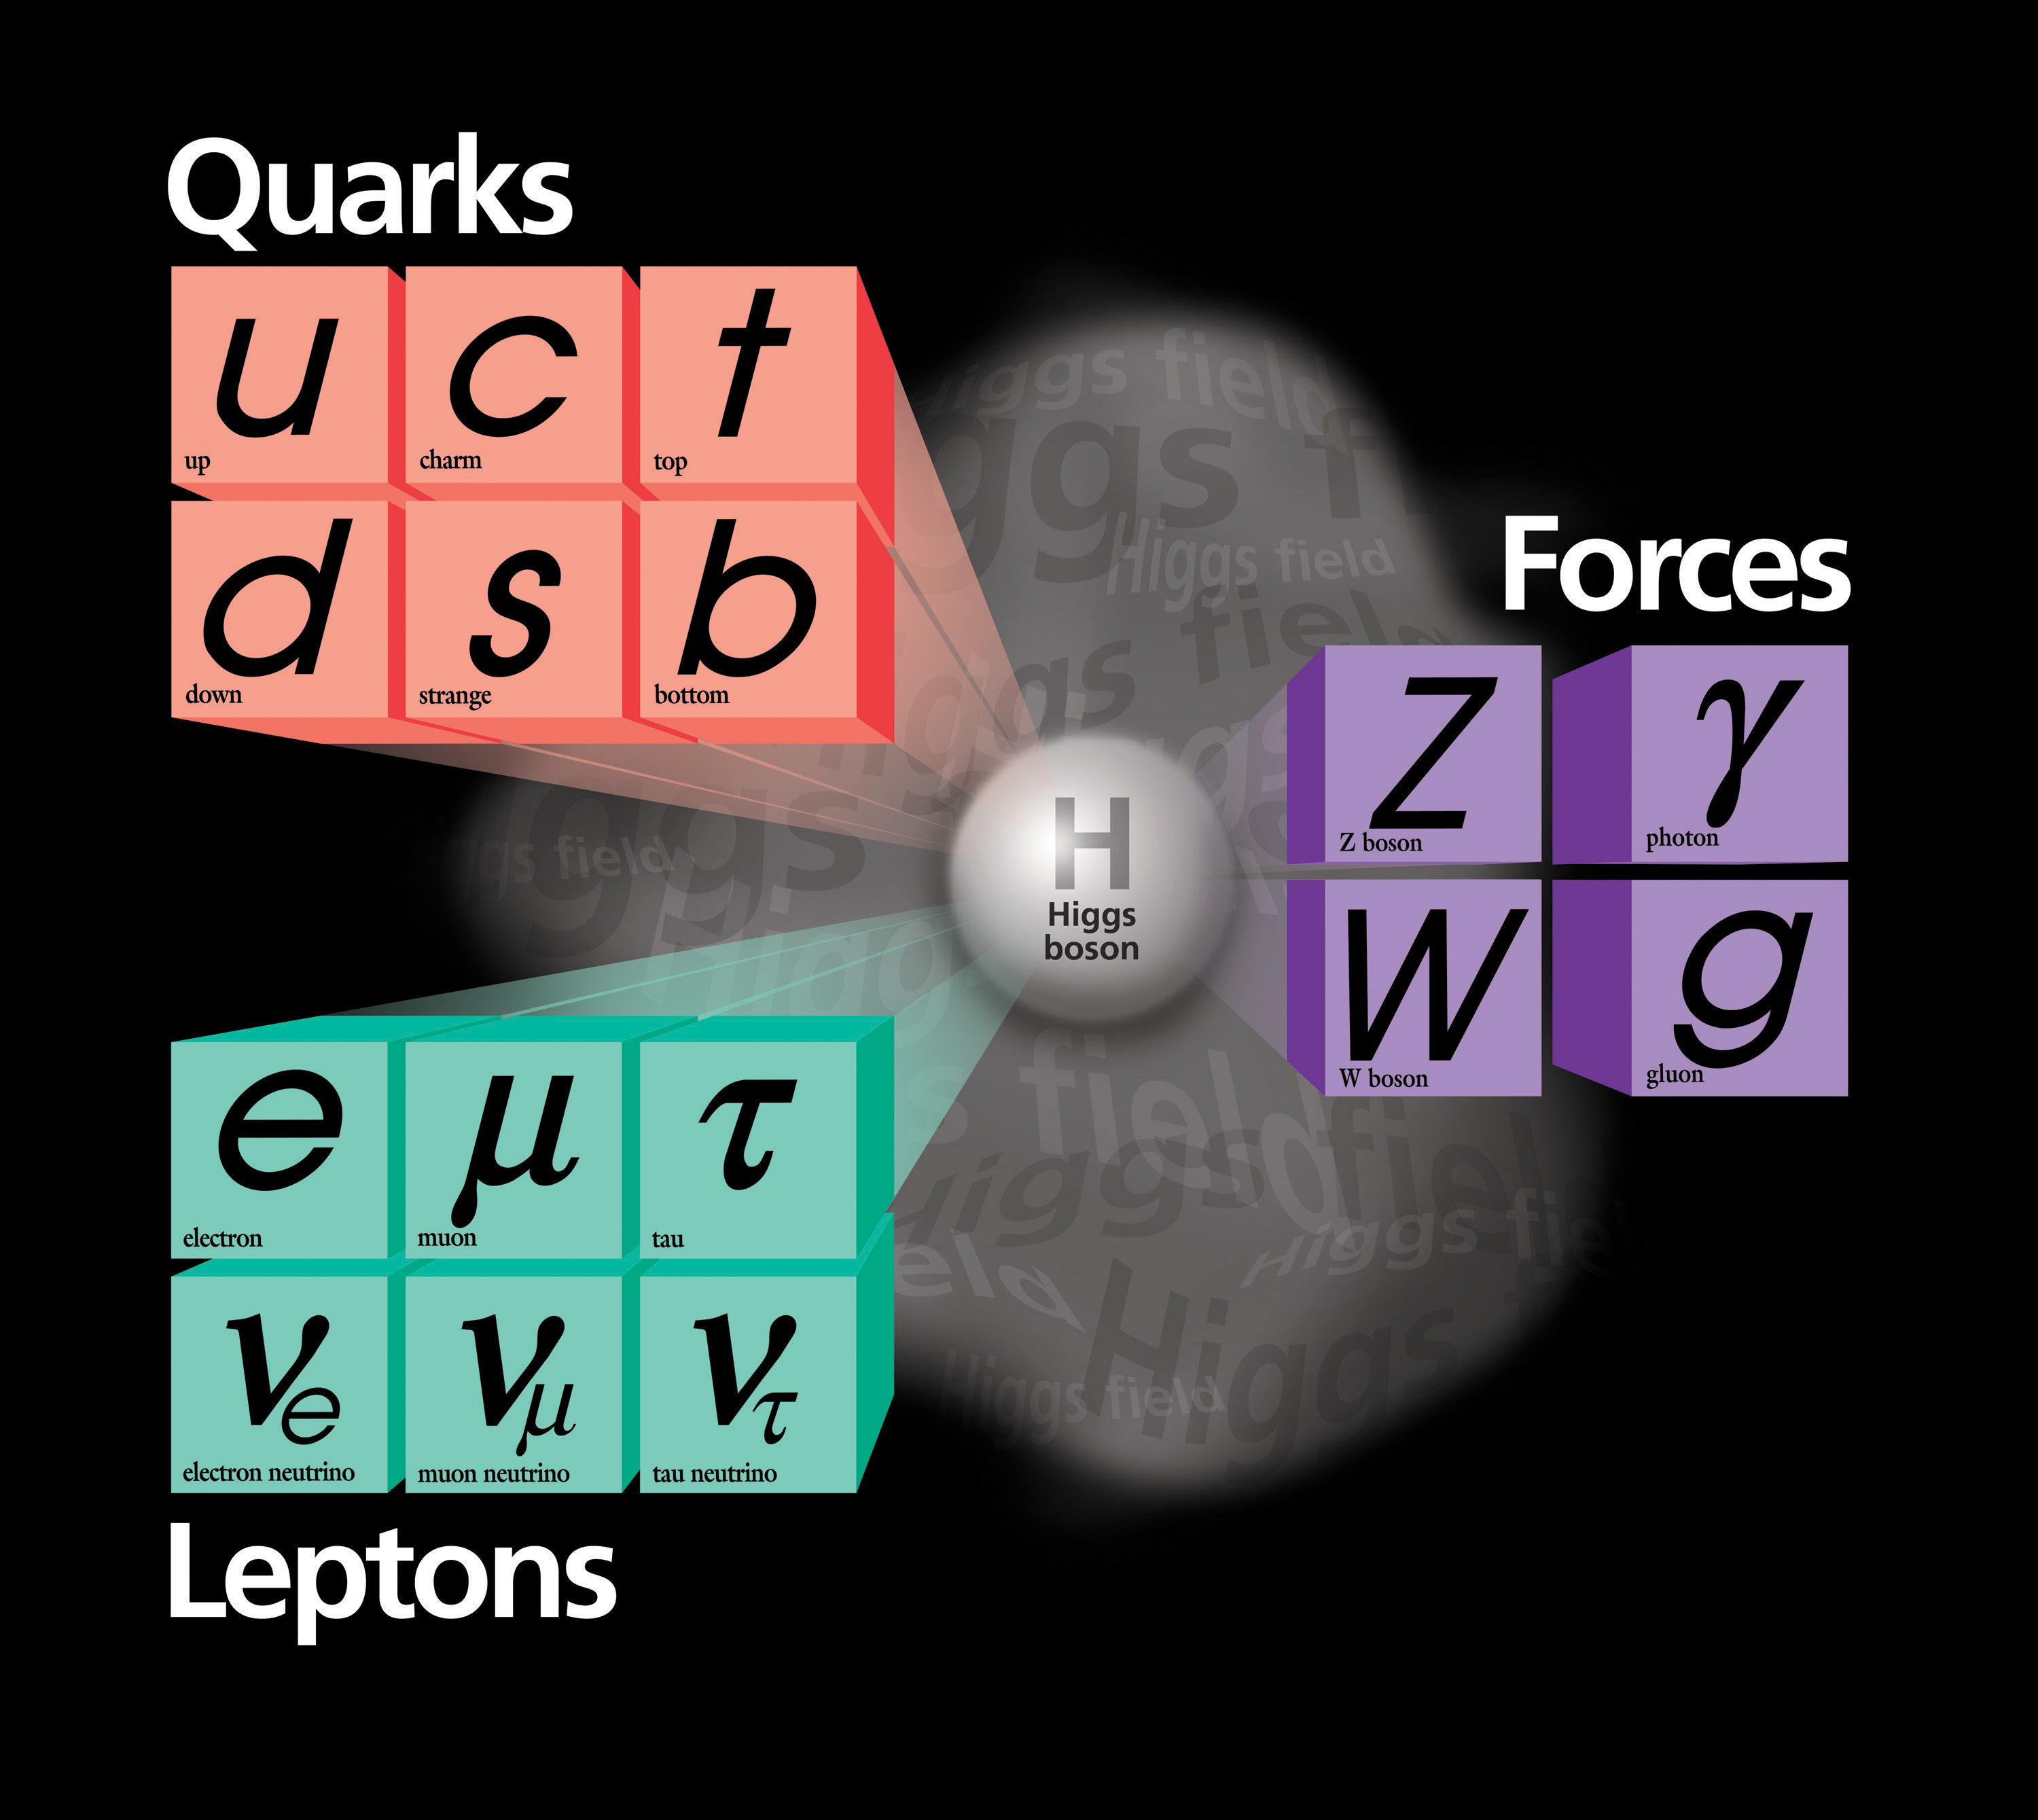
\includegraphics[width=0.6\textwidth]{plots/intro/Higgs_SM.jpeg}
\caption{Table of elementary particles: quarks and leptons (spin-1/2) are shown on the left,
the gauge bosons (spin-1) on the right, in the center the Higgs boson (spin-0).
\label{fig:parttable}}

\end{figure}

The particles within each of the weak isodoublets differ in terms of their
mass and electric charge, making them distinguishable.
 Therefore the weak isospin interaction is
 not an observed symmetry of nature, but it was clearly present
in some form given the structure of the particles table. 
In order to explain the physically observed masses and charges of elementary
 particles we need to introduce electroweak symmetry breaking, a central concept
of the SM that transforms the
weak isospin and hypercharge interactions into the well known weak and electromagnetic forces.



\subsection{The Higgs Mechanism}

What happens if a particle field takes on a non-zero expectation value in vacuum? Depending on the
quantum numbers of this non-zero field, the vacuum will not necessarily be invariant under
all symmetries of the Lagrangian. That is what is postulated by the Higgs mechanism
\cite{Anderson:1963pc,Englert:1964et,Higgs:1964pj}, where
the existence of a scalar field with non-zero vacuum expectation value
reduces the gauge symmetries of the physical 
vacuum from $\text{SU}(3)_\text{C} \times \text{SU}(2)_\text{L} \times \text{U}(1)_\text{Y}$
down to $\text{SU}(3)_\text{C} \times \text{U}(1)_\text{EM}$, thus leaving the physical vacuum invariant under
only the color and electric charges. 
The $\text{U}(1)_\text{EM}$ symmetry group requires the existence of a massless
gauge boson, the photon ($\gamma$), as the carrier of electromagnetic force.
After symmetry breaking the gauge bosons mix to form weak and electromagnetic fields:
\begin{equation}
W_{\mu}^{\pm}=\frac{1}{\sqrt{2}}\left( W_{\mu}^1 \mp W_{\mu}^{2}\right),
\end{equation}
\begin{equation}
Z_{\mu}=\cos\theta_W W_{\mu}^3-\sin\theta_W B_{\mu},
\end{equation}
\begin{equation}
A_{\mu}=\sin\theta_W W_{\mu}^3+\cos\theta_W B_{\mu}
\end{equation}
where $\theta_W$ is the weak mixing angle defined as $\theta_W=\tan^{-1} g^{'}/g$, where $g$ 
and $g^{'}$ are the coupling constants of $\text{SU}(2)_\text{L}$ and $\text{U}(1)_\text{Y}$, respectively; $A_{\mu}$ is the 
massless electromagnetic photon field ($\gamma$); and $W_{\mu}^{\pm}$ and $Z_{\mu}$ are the charged 
and neutral weak fields. The mechanism requires the introduction of a complex
scalar Higgs doublet. The potential introduced by this field breaks part of the electroweak
 gauge symmetry,
after which only one neutral Higgs scalar $H$ remains. As a result, 
the $W^{\pm}$ and $Z$ acquire masses and the photon remains massless.

\section{Open questions and physics beyond the SM}

At the current stage all the parameters of the SM have been experimentally measured,
the last being the Higgs mass, and the
self-consistency of the theory has been tested with electroweak fits \cite{Baak:2013ppa}.
%The SM is consistent with essentially all the partcile physics phenomena.
Thus far, the SM proves to be self-consistent and exhibits good agreement between
predicted and measured observables. More precise measurements and theoretical calculations
are needed in order to emphasize weak points of the SM and thus
find indirect hints of new physics.
Despite its consistency, the SM remains incomplete as it cannot answer some fundamental 
questions. I list a few of them below:
\begin{itemize}
 \item {\it the hierarchy problem} --- the gravitational interaction becomes strong only at the 
Planck scale, $10^{19}$ GeV, which is much above the electroweak scale of $\sim 100$ GeV. 
In the SM the Higgs boson mass 
depends on quantum corrections on the order of the Planck scale, unless there
exists some cancellation mechanism, such as supersymmetry \cite{Martin:1997ns}, extra dimensions
\cite{ArkaniHamed:1998rs,Zee:2003mt}, or fine-tuning; 
 \item {\it the grand unification of interactions} --- at energies of $\sim 10^{16}$ GeV
the coupling constants of the SM gauge symmetries become approximately equal, which suggests
there may exists a single gauge symmetry (typically SO(10)) with just one coupling constant
\cite{Georgi:1974sy,Buras197866};
 \item {\it the dark matter} --- it is not known how to incorporate the observed
 dark matter into the theory (should it consists of particles) \cite{Bertone2005279};
 \item {\it the neutrino masses} --- the nature of the neutrino mixing and masses is yet to be
determined as well as whether they follow Dirac or Majorana statistics \cite{Fukuda:1998fd};
 \item {\it the number of fermion generations} --- it is unknown why are there three generations
of fermions \cite{Decamp:1989tu};
 \item {\it the matter-antimatter asymmetry} --- the observable imbalance between the matter and
antimatter in the observable universe hasn't yet been explained \cite{Fukugita:1986hr};
 \item {\it the vacuum energy} --- the SM vacuum
energy density is many orders of magnitude higher when compared to astrophysical measurements
of the cosmological constant \cite{Sahni:1999gb,Rugh2002663};
\end{itemize}
Moreover, the SM involves 19 parameters, whose values are experimentally determined, but not derived from
first principles.
To overcome some of the above difficulties many theories beyond the SM have been
proposed, such as Supersymmetry (SUSY), Grand Unified Theories (GUT), extra dimensions and others.
To date none of them has been experimentally confirmed, nonetheless the searches continue.
In the next section an alternative extension of the SM known as Hidden Valleys 
is introduced. 

\section{Hidden Valleys and Long-Lived particles}

In many theories like string theory, supersymmetry, grand unification theories etc.
 one encounters large symmetry groups, which imply the existence of
new particles. In these theories the SM symmetry group $\text{SU}(3)_\text{C} \times \text{SU}(2)_\text{L} \times \text{U}(1)_\text{Y}$ 
 that we observe at the electroweak scale is only a part of a bigger picture.
The new interactions between
both ordinary and new matter will arise from the larger symmetry groups,  and  
the new states are usually
assumed to have masses around the Grand Unification or the Planck scales. However, it is not unreasonable
to assume that some of the new particles are lighter, much closer to the electroweak scale,
but there is some barrier that has thus far prevented us from finding them. A new sector
of relatively light particles not accessible because of some high energy barrier is called 
a Hidden Valley \cite{Strassler:2006im,Strassler:2006qa}.
Although, the relevant mass scale of the Hidden Valley is not well
specified, it is interesting to study scenarios that may produce visible signals within 
the reach of the LHC.
A good analogy from the SM are 
the neutrinos, which are somewhat hidden by only interacting via the massive $W$ and $Z$ bosons.
There is no reason why the new particles cannot be hidden also. 

In Hidden Valley models, the SM gauge group $G_{SM}$ is extended by a symmetry 
group of the hidden sector $G_v$. 
All SM particles carry no charges in $G_v$, while
all the new particles ($v$-particles) in the hidden sector are charged in $G_v$ and neutral 
in $G_{SM}$. Higher dimension operators (induced perhaps by a Higgs particle, a $Z^{'}$ or
a lightest supersymmetric particle) allow interaction between SM
fields and the $v$-particles.
One typically assumes that the $G_v$ is a confining, non-abelian group with the
$v$-confinement scale $\Lambda_v$, resembling the SM color group,
therefore $v$-particles assemble themselves into $G_v$-neutral $v$-hadrons.
The $v$-particles may then decay, again via higher dimension operators, to gauge invariant 
combinations of SM particles. The interactions between the SM and Hidden Valley sector are
schematically presented in Fig.~\ref{fig:hv}. 

\begin{figure}[htbp]
\centering
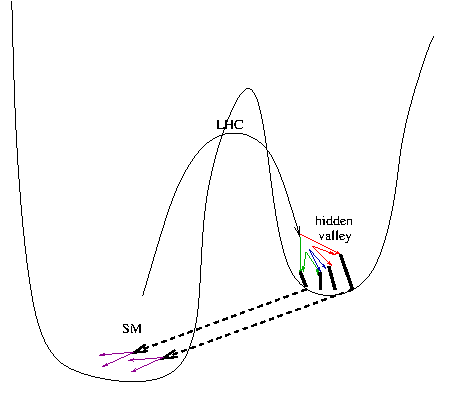
\includegraphics[width=0.6\textwidth]{plots/intro/hiddenvalley.pdf}
\caption{Schematic view of production and decay of v-hadrons. If with the energies
available at the LHC we may penetrate the barrier and produce v-hadrons, some of them may
decay back to SM particles. \label{fig:hv}}
\end{figure}

There is not a clear minimal representative for Hidden Valley models, but
many phenomena are common for a typical $v$-sector. Some examples are listed
\cite{Strassler:2006ri,Han:2007ae,Strassler:2008fv}:
\begin{itemize}
\item $v$-hadron production multiplicites at the LHC may be large, especially if $\Lambda_v\ll1$\TeV;
\item some $v$-hadrons may be stable, providing dark matter candidates and missing energy signals,
while others decay to neutral combinations of SM particles;
\item decay lifetimes can vary over many orders of magnitude, some of the $v$-particles may produce
displaced vertices;
\item some $v$-hadrons decay preferentially to heavy flavor, while others decay more democratically
to $f\bar{f}$ states ($f$ is any SM fermion), or $f\bar{f}$ plus another $v$-hadron or other final
states.
\end{itemize}

If the $v$-particles can be produced at the LHC, they can be detected via missing energy 
searches, lepton resonance searches, or displaced vertex searches. In this dissertation,
we focus on a particular signature where a long-lived $v$-particle 
decays to quark-antiquark pairs~($\qq$) at a displaced vertex,
 while we study all SM quark flavors except the top flavor. Due to the color confinement 
phenomenon, quarks
will hadronize into jets, therefore we will use the term {\it quark} and  {\it jet} as 
 equivalent from the detection perspective,
while a {\it quark-antiquark pair} will also be called a {\it dijet}.
The analysis presented in the next chapters is potentially sensitive 
to any heavy particle that decays into a pair of jets 
 at a displaced vertex. However, we study the search sensitivity and optimise the selection
 using a 
specific Hidden Valley
model as our benchmark. In this model a long-lived, spinless, neutral
exotic particle \X decays to $\qq$,
 the \X is pair-produced in the decay of a non-SM Higgs boson, i.e.  \Higgs~$\to
2$\X~, \X~$\to \qq$ \cite{Strassler:2006ri}, and 
the non-SM Higgs boson is produced through gluon-gluon
fusion. 

Several other models of new physics predict the existence of massive, 
long-lived particles which could
manifest themselves through non-prompt decays to dijets. Such scenarios arise, for example,
in various supersymmetric (SUSY) scenarios such as ``split SUSY''
\cite{Hewett:2004nw} or SUSY with very weak R-parity violation \cite{Barbier:2004ez}, 
or \Zprime models
that contain long-lived neutrinos~\cite{Basso:2008iv}. 
The outstanding feature, common in the above models,
is the existence of a massive long-lived particle that decays to {\it at least} two
quark jets. The search is therefore designed to look for pairs of hadronic jets
 that emerge from a common displaced vertex, thus allowing 
for multiple interpretations.

\section{Previous and present searches}

The CDF and D0 collaborations at the Tevatron have performed searches for metastable particles decaying to $b$-quarks
\cite{Aaltonen:2011rja, Abazov:2009ik}.
These searches are sensitive to a smaller kinematic phase space region than CMS and explore
lower masses of the exotic particles. The ATLAS collaboration
at the LHC has performed searches that are sensitive to decay lengths of 1--20\unit{m} by exploiting the ATLAS muon
 spectrometer \cite{ATLAS:2012av}, whilst the search presented here is sensitive to decay lengths 
typically below 1~m.
 The ATLAS search required the long-lived particles to be pair-produced,
while our search
is also sensitive to single or associated production.
A previous search by the CMS collaboration for long-lived particles in a similar phase-space region utilized leptonic decay channels~\cite{Chatrchyan:2012jna}.

The search presented here has been published as a CMS Physics Analysis Summary 
\cite{CMS-PAS-EXO-12-038}. Its journal publication is under way.
%An additional interpretation in terms of a SUSY model with R-parity
%violation is currently under study.
